% !TEX TS-program = pdflatex
% !TEX encoding = UTF-8 Unicode

% This is a simple template for a LaTeX document using the "article" class.
% See "book", "report", "letter" for other types of document.

\documentclass[11pt]{article} % use larger type; default would be 10pt

\usepackage[utf8]{inputenc} % set input encoding (not needed with XeLaTeX)

%%% PAGE DIMENSIONS
\usepackage{geometry} % to change the page dimensions
\geometry{a4paper} % or letterpaper (US) or a5paper or....

\usepackage{graphicx} % support the \includegraphics command and options

\usepackage{amssymb}
\usepackage{amsmath}
%%% PACKAGES
\usepackage{booktabs} % for much better looking tables
\usepackage{array} % for better arrays (eg matrices) in maths
\usepackage{paralist} % very flexible & customisable lists (eg. enumerate/itemize, etc.)
\usepackage{verbatim} % adds environment for commenting out blocks of text & for better verbatim
\usepackage{subfig} % make it possible to include more than one captioned figure/table in a single float
% These packages are all incorporated in the memoir class to one degree or another...

%%% HEADERS & FOOTERS
\usepackage{fancyhdr} % This should be set AFTER setting up the page geometry
\pagestyle{fancy} % options: empty , plain , fancy
\renewcommand{\headrulewidth}{0pt} % customise the layout...
\lhead{}\chead{}\rhead{}
\lfoot{}\cfoot{\thepage}\rfoot{}

%%% SECTION TITLE APPEARANCE
\usepackage{sectsty}
\allsectionsfont{\sffamily\mdseries\upshape} % (See the fntguide.pdf for font help)
% (This matches ConTeXt defaults)

%%% ToC (table of contents) APPEARANCE
\usepackage[nottoc,notlof,notlot]{tocbibind} % Put the bibliography in the ToC
\usepackage[titles,subfigure]{tocloft} % Alter the style of the Table of Contents
\renewcommand{\cftsecfont}{\rmfamily\mdseries\upshape}
\renewcommand{\cftsecpagefont}{\rmfamily\mdseries\upshape} % No bold!
\usepackage{graphicx}
\graphicspath{ {./pings/} }

\usepackage{amsmath}
\DeclareMathOperator*{\argmax}{arg\,max}
\DeclareMathOperator*{\argmin}{arg\,min}

\newcount\colveccount
\newcommand*\colvec[1]{
        \global\colveccount#1
        \begin{pmatrix}
        \colvecnext
}
\def\colvecnext#1{
        #1
        \global\advance\colveccount-1
        \ifnum\colveccount>0
                \\
                \expandafter\colvecnext
        \else
                \end{pmatrix}
        \fi
}

%%% END Article customizations

%%% The "real" document content comes below...

\title{Macro PS7}
\author{Michael B. Nattinger\footnote{I worked on this assignment with my study group: Alex von Hafften, Andrew Smith, and Ryan Mather. I have also discussed problem(s) with Emily Case, Sarah Bass, and Danny Edgel.}}

%\date{} % Activate to display a given date or no date (if empty),
         % otherwise the current date is printed 

\begin{document}
\maketitle

\section{Question 1}
The planner maximizes utility subject to the resource constraint:
\begin{align*}
\max_{c_t^t,h_t,c_{t}^{t-1}} ln(c_t^t) + \alpha h_t + \beta c_{t}^{t-1}\\
\text{s.t. } c_t^t + c_{t}^{t-1} = y\\
\text{and } h_t = H^s
\end{align*}
Clearly we can use the resource constraints to find that $h_t = H^s =1$, and then solve for $c_t^t = y - c_t^{t-1}.$ We then rewrite our optimization problem as:
\begin{align*}
\max_{c_{t}^{t-1}} ln(y - c_t^{t-1}) + \alpha  + \beta c_{t}^{t-1}
\end{align*}
Taking FOCs:
\begin{align*}
\frac{d u}{dc_t^{t-1}} = 0 &\Rightarrow \beta = \frac{1}{y-c_t^{t-1}} \Rightarrow c_{t}^{t-1} = y - \frac{1}{\beta}\\
&\Rightarrow c_t^t = y - (y - \frac{1}{\beta}) =  \frac{1}{\beta}
\end{align*}
\section{Question 2}
\subsection{Part A}
The young agents face the following optimization problem:
\begin{align*}
\max_{c_t^t,h_t,c_{t}^{t-1}} ln(c_t^t) + \alpha h_t + \beta c_{t+1}^{t}\\
\text{s.t. } c_t^t + p_t h_t \leq y\\
\text{and } c_{t+1}^t \leq p_{t+1}h_{t}
\end{align*}

\subsection{Part B}

Markets clearing in the goods and housing market implies the following:
\begin{align*}
c_t^t + c_{t}^{t-1} &= y\\
h_t = H^s &= 1
\end{align*}
\subsection{Part C}
A competitive equilibrium is a set of allocations and prices such that agents optimize and markets clear.
\subsection{Part D}
Utility is strictly increasing in consumption, so the budget constraints will hold with equality and we can substitute $c_t^t = y - p_th_t,c_{t+1}^t = p_{t+1}h_t$ into the maximization problem and take first order conditions:
\begin{align*}
&\max_{h_t} ln(y - p_th_t) + \alpha h_t + \beta p_{t+1}h_t\\
\frac{du}{dh_t} = 0 &\Rightarrow \frac{p_t}{y-p_th_t} = \alpha + \beta p_{t+1}\\
&\Rightarrow h_t = \frac{y}{p_t} - \frac{1}{\alpha + \beta p_{t+1}}\\
&\Rightarrow c_t^t =  \frac{p_t}{\alpha + \beta p_{t+1}} \\
&\Rightarrow c_{t+1}^t =  \frac{yp_{t+1}}{p_t} - \frac{p_{t+1}}{\alpha + \beta p_{t+1}}
\end{align*}

We should verify that consumption and housing are nonnegative. This will be the case so long as $p_t,p_{t+1}$ are positive and $\frac{y}{p_t} > \frac{1}{\alpha + \beta p_{t+1}}.$

\subsection{Part E}
From the market clearing conditions,
\begin{align*}
\frac{y}{p_t} - \frac{1}{\alpha + \beta p_{t+1}} = 1 &\Rightarrow p_{t+1} = \frac{p_t}{\beta(y-p_t)} - \frac{\alpha}{\beta}\\
&\Rightarrow c_t^t = y - p_t,c_{t+1}^t = p_{t+1}
\end{align*}

Note that this also implies the second condition for consumption to be nonnegative. Now we should check the price condition:

\begin{align*}
0\leq p_{t+1} = \frac{p_t}{\beta(y-p_t)} - \frac{\alpha}{\beta} \Rightarrow p_t\geq \frac{\alpha}{1+\alpha}y.
\end{align*}
We are given that $p_t<y$ so $ \frac{\alpha}{1+\alpha}y \leq p_t \leq y$.

Below is the graph of $p_{t+1}$ vs $p_t$. 

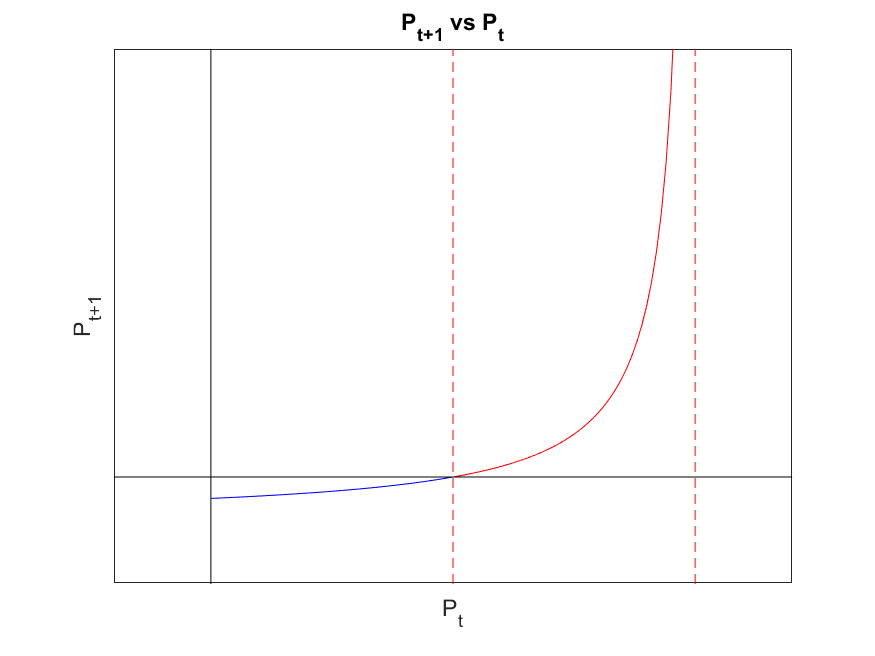
\includegraphics{fig1}
In the above figure, we can see $p_{t+1}$ as a function of $p_t$. Due to the nonnegativity constraints, the allowed values of $p_{t+1}$ are positive, and are drawn in red. The positive region is within the dashed red lines, indicating $\frac{\alpha}{1+\alpha}y\leq p_t\leq y$.

\subsection{Part F}
In the steady state, $\bar{p} = p_t = p_{t+1} \Rightarrow \bar{p} = \frac{\bar{p}}{\beta(y-\bar{p})} - \frac{\alpha}{\beta}$
\begin{align*}
&\Rightarrow 0 =\bar{p} - \alpha(y - \bar{p}) - \bar{p}\beta(y - \bar{p})\\
&\Rightarrow 0 = \beta \bar{p}^2 +(1+\alpha - \beta y)\bar{p} - \alpha y \\
&\Rightarrow \bar{p} = \frac{-(1+\alpha - \beta y) \pm \sqrt{(1+\alpha - \beta y)^2 +4\beta \alpha y} }{2\beta} 
\end{align*}
The nonnegativity constraint rules out the negative $\bar{p}$ value so $\bar{p} = \frac{-(1+\alpha - \beta y) + \sqrt{(1+\alpha - \beta y)^2 +4\beta \alpha y} }{2\beta}.$
\subsection{Part G}
Since in the steady state $p_t = \bar{p} =  \frac{-(1+\alpha - \beta y) \pm \sqrt{(1+\alpha - \beta y)^2 +4\beta \alpha y} }{2\beta} $, $\bar{c}_t^t =\bar{p} =  \frac{-(1+\alpha - \beta y) \pm \sqrt{(1+\alpha - \beta y)^2 +4\beta \alpha y} }{2\beta}, \\ \bar{c}_{t+1}^t = y - \bar{p} = y- \frac{-(1+\alpha - \beta y) \pm \sqrt{(1+\alpha - \beta y)^2 +4\beta \alpha y} }{2\beta} $ which is not the planner's solution of $c_t^t = \frac{1}{\beta}, c_{t+1}^t = y - \frac{1}{\beta}$. However, in both equilibria the housing is the same due to market clearing in the housing market: $\bar{h} = 1 = h_t$.
\end{document}
